\stfhIndex{I157}{PSSyingshe}{PSS 映射（PSS map）}
\section{PSS 映射及其同构性质}
\label{sec:pss-map-isomorphism}

令 $f:M\to\mathbb R$ 为 $M$ 上的背景\personMorse{}函数，$H=H(t,x)$，$J=J(t,x)$。
PSS 映射的目标是在 $f$ 的\personMorse{}同调与 $(H,J)$ 的\personFloer{}同调之间建立同构。

PSS 映射构造所用的模空间之一，是方程~\eqref{eq:20-asymptotic-perturbed-cr} 在亏格
$0$ 定义域上的解空间：定义域有一个可正可负的穿孔，以及一个充当
$\dot\Sigma\cong\mathbb C$ 原点的标记点。我们先引入具有任意多个正穿孔、负穿孔和
标记点的这类一般模空间。

\subsection{PSS 映射模空间的定义}

本小节回忆 (PSS96) 中两个 PSS 映射 $\Phi,\Psi$ 的定义，不过我们使用 $-f$ 而非
$f$ 的\personMorse{}闭链代表 $M$ 的同调。特别地，\personMorse{}闭链的分次为
\[
 \operatorname{Index}_{(-f)}(p)=2n-\operatorname{Index}_f(p),
\]
这与作者在 (Oh05c)--(Oh06a) 和 (OhZ11b) 等论文中使用的约定一致。因此，我们将
构造量子上同调与\personFloer{}同调之间的同构
$QH^*(M)\to HF_*(H,J)$。

令 $(C_*,\partial)$ 是 $M$ 上任意同调为奇异同调 $H_*(M)$ 的链复形。取
$C_*$ 为 $(-f,g_{J_0})$ 的\personMorse{}同调复形
\[
 \bigl(CM_*(-f),\partial^{\mathrm{Morse}}_{(-f,g_{J_0})}\bigr)
 \cong\bigl(CF_*(f),\partial^{\mathrm{Floer}}_{(f,J_0)}\bigr),
\]
其中 $\|f\|_{C^2}$ 充分小。在此约定下，$-f$ 的负梯度解对应于作用量泛函
$\mathcal A_f$ 的负梯度流解。

令 $\dot\Sigma_+$ 为带一个标记点 $o_+$ 和一个正穿孔 $e_+$ 的\personRiemann{}球面。
等同 $\dot\Sigma_+\setminus\{o_+\}\cong\mathbb R\times S^1$，以 $(\tau,t)$ 表示
相应坐标，使 $\{+\infty\}\times S^1$ 对应 $e_+$。坐标 $(\tau,t)$ 只在
$\mathbb R\times S^1\cong\mathbb C^*$ 的作用下确定：
\[
 (\tau,t)\longmapsto(\tau+a,t+b).
\]
考虑单形式 $K_+\in\Omega^1(\dot\Sigma,\operatorname{ham}(M,\omega))$，它可写为
\begin{equation}
 K_+=\begin{cases}
 0,&\text{在 }o_+\text{ 附近},\\
 H_+(t,x)dt,&\text{在 }e_+\text{ 附近},
 \end{cases}
 \label{eq:20-k-plus}
\end{equation}
其中 $H_+$ 是某个哈密顿量。令 $z_+=z_+(t)$（$t\in S^1$）为 $H_+$ 的非退化周期
轨道，$[z_+,w_+]$ 为 $z_+$ 到 $\widetilde{\mathcal L}_0(M)$ 的一个提升。考虑模空间
\stfhIndex{I012}{00-m-kplus}{$\mathcal M(K^+,J^+;[z^+,w^+];A^+)$}
\[
 \begin{aligned}
 \mathcal M(K_+,J_+;[z_+,w_+];A_+)=\{u:\dot\Sigma\to M\mid{}
 &\overline\partial_{(K_+,J_+)}u=0,\\
 &u(+\infty,t)=z_+(t),\ [u\#w_+]=A_+\},
 \end{aligned}
\]
其中 $A_+\in H_2(M,\mathbb Z)$ 落在\personHurewicz{}映射
$\pi_2(M)\to H_2(M,\mathbb Z)$ 的像中。
\footnote{译者注：原书把这里的 Hurewicz map 误写成 Hurwitz map；译文按映射
$\pi_2(M)\to H_2(M,\mathbb Z)$ 的标准名称改正。}
对通有的 $J_+$ 或 $K_+$，该模空间正则，且
\[
 \operatorname{Index}D_u\overline\partial_{(K_+,J_+)}
 =n-\mu_{H_+}([z_+,w_+])+2c_1(A_+).
\]
类似地，定义
\stfhIndex{I013}{00-m-kminus}{$\mathcal M(K^-,J^-;[z^-,w^-];A^-)$}
\[
 \begin{aligned}
 \mathcal M(K_-,J_-;[z_-,w_-];A_-)=\{u:\dot\Sigma\to M\mid{}
 &\overline\partial_{(K_-,J_-)}u=0,\\
 &u(-\infty,t)=z_-(t),\ [\overline w_-\#u]=A_-\},
 \end{aligned}
\]
其中 $A_-$ 与 $A_+$ 类似，并有
\[
 \operatorname{Index}D_u\overline\partial_{(K_-,J_-)}
 =n+\mu_{H_-}([z_-,w_-])+2c_1(A_-).
\]

若用 $-f$ 的\personMorse{}同调表示 $H_*(M)$，则可把量子同调 $QH_*(M)$ 表示为
$C_*(-f)\otimes\Lambda_\omega$ 的同调，其中 $C_*(-f)$ 是由 $f$ 的临界点生成的
$-f$ \personMorse{}同调链复形。$[p]q^{-A}$ 的分次为
$\mu_{(-f)}(p)-2c_1(A)$，其中 $[p]\in C_*(-f)$，而 $\mu_{(-f)}(p)$ 是 $-f$ 在
$p$ 处的\personMorse{}指标。
\footnote{译者注：原书末句印作“$f$ 在 $p$ 处的 Morse 指标”，但记号及本段首句均为
$\mu_{(-f)}$；译文据此补出负号。}

我们先定义相应链映射
$\Phi:C_*(-f)\otimes\Lambda_\omega\to CF_*(H)$，以构造同构
\[
 \Phi_*:QH_k(M)[n]\;(=QH_{k+n}(M))\longrightarrow HF_k(H,J).
\]
它在生成元 $[p]$ 上定义为
\[
 \Phi:[p]\longmapsto
 \sum_{[z_+,w_+]\in\widetilde{\operatorname{Per}}(H_+)}
 \#\bigl(\mathcal M(p,[z_+,w_+];A_+)\bigr)[z_+,w_+]q^{-A_+},
\]
再对 $\Lambda_\omega$ 线性延拓。粗略地说，
$\mathcal M(p,[z_+,w_+];A_+)$ 由从临界点 $p$ 发出、终止于周期轨道 $z_+$，且
$[u\#w_+]=A_+$ 于 $\Gamma$ 的“尖刺圆盘”组成。精确定义为
\stfhIndex{I015}{00-m-p-zplus}{$\mathcal M(p,[z^+,w^+];A^+)$}
\[
 \begin{aligned}
 \mathcal M(p,[z_+,w_+];A_+)=\{(\chi_+,u_+)\mid{}
 &u_+:\dot\Sigma_+\to M,\ [u_+\#w_+]=A_+,\\
 &u(+\infty,t)=z_+(t),\ \overline\partial_{(K_+,J_+)}u_+=0,\\
 &\dot\chi_+=\nabla f(\chi_+),\ \chi_+(-\infty)=p,
 \ \chi_+(0)=u_+(o_+)\}.
 \end{aligned}
\]
施加指标条件，使此空间成为可作代数计数“$\#$”的零维定向流形：
\[
 n-\mu([z_+,w_+])+2c_1(A_+)+(2n-\mu(p))-2n=0,
\]
亦即
\[
 \mu([z_+,w_+])=n-(\mu(p)-2c_1(A_+)).
\]
\footnote{译者注：原书第一式把 $+2c_1(A_+)$ 排在 $\mu$ 的括号内，类型上会把整数
加到提升轨道后再取指标；第二式及前述\personFredholm{}指标表明它应在 $\mu$ 外，译文据此
排写。}
粘合论证说明 $\Phi$ 是链映射，因而下降到同调，得到 (Pi94), (PSS96) 引入的 PSS
映射 $\Phi_*:QH_*(M)\to HF_*(H,J)$。

接下来在链层定义 $\Phi$ 的逆
\[
 \Psi_*:HF_*(H,J)\longrightarrow QH_*(M).
\]
对任意 $[z_-,w_-]\in\widetilde{\operatorname{Per}}(K_-)$，定义
$\Psi:CF_*(H)\to C_*(-f)\otimes\Lambda_\omega$：
\stfhIndex{I014}{00-m-zminus-p}{$\mathcal M([z^-,w^-],p;A^-)$}
\[
 \Psi:[z_-,w_-]\longmapsto
 \sum_{p\in\operatorname{Crit}(-f),\ A_-\in\pi_2(M)}
 \#\mathcal M([z_-,w_-],p;A_-)\,p\otimes q^{-A_-}.
\]
\footnote{译者注：原书把此处定义域印作 $CF_*(M)$，但本段输入是 $H$ 的提升周期轨道，
且所构造的是 $HF_*(H,J)$ 上映射；译文写作 $CF_*(H)$。}
如图~\ref{fig:20-pss-maps} 所示，$\mathcal M([z_-,w_-],p;A_-)$ 由从周期轨道
$z_-$ 发出并终止于临界点 $p$ 的“尖刺圆盘”组成：
\[
 \begin{aligned}
 \mathcal M([z_-,w_-],p;A_-)=\{(u_-,\chi_-)\mid{}
 &u_-:\dot\Sigma_-\to M,\ [\overline w_-\#u_-]=A_-,\\
 &u(-\infty,t)=z_-(t),\ \overline\partial_{(K_-,J_-)}u_-=0,\\
 &\dot\chi_-=\nabla f(\chi_-),\ \chi_-(+\infty)=p,
 \ \chi_-(0)=u_-(o_-)\}.
 \end{aligned}
\]

\begin{figure}[htbp]
 \centering
 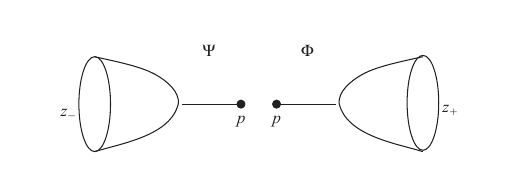
\includegraphics[width=.62\textwidth]{chapters/ch20-pants-product/figures/figure-20-1.png}
 \caption{PSS 映射 $\Psi$ 与 $\Phi$。}
 \label{fig:20-pss-maps}
\end{figure}

这里同样施加指标条件
\[
 \mu_{H_-}([z_-,w_-])=n-(\mu_{(-f)}(p)-2c_1(A_-)),
\]
使 $\mathcal M([z_-,w_-],p;A_-)$ 成为零维（可定向）流形。同样的延拓映射论证说明
$\Psi$ 是链映射，故在同调上诱导同态。

\stfhIndex{I028}{Jueretuihua}{绝热退化（adiabatic degeneration）}
\subsection{\personFloer{}模空间的绝热退化}

本小节描述 (OhZ11b) 建立的主要绝热粘合结果，不深入高度非平凡的分析细节；完整
细节见原文。在 $U_\pm$ 上用给定解析坐标 $z=e^{2\pi(\tau+it)}$，固定函数
\begin{equation}
 \kappa^+(\tau)=\begin{cases}0,&|\tau|\leq1,\\1,&|\tau|\geq2,
 \end{cases}
 \label{eq:20-kappa-plus}
\end{equation}
并令 $\kappa^-(\tau)=\kappa^+(-\tau)$。置
$\kappa_\epsilon^+(\tau)=\kappa^+(\tau-R(\epsilon)+1)$、
$\kappa_\epsilon^-(\tau)=\kappa_\epsilon^+(-\tau)$。容易看出
\begin{equation}
 \kappa_\epsilon^+(\tau)=\begin{cases}
 1,&\tau\geq R(\epsilon)+1,\\0,&\tau\leq R(\epsilon),
 \end{cases}
 \qquad
 \kappa_\epsilon^-(\tau)=\begin{cases}
 1,&\tau\leq-R(\epsilon)-1,\\0,&\tau\geq-R(\epsilon).
 \end{cases}
 \label{eq:20-kappa-epsilon-pm}
\end{equation}
再把它们在坐标卡 $U_\pm$ 外延拓为零。选取 $R=R(\epsilon)$，使
\begin{equation}
 \epsilon R(\epsilon)\longrightarrow0\qquad(\epsilon\to0).
 \label{eq:20-epsilon-r-normalization}
\end{equation}
绝热退化论证中的归一化步骤将用到这一选取。

还取截断函数 $\kappa_\epsilon^0:\mathbb R\to[0,1]$，满足
\begin{equation}
 \kappa_\epsilon^0(\tau)=\begin{cases}
 1,&|\tau|\leq R(\epsilon)-1,\\0,&|\tau|\geq R(\epsilon),
 \end{cases}
 \label{eq:20-kappa-zero}
\end{equation}
以及
\begin{equation}
 |(\kappa_\epsilon^0)'(\tau)|\leq2
 \qquad\text{当 }R(\epsilon)-1\leq|\tau|\leq R(\epsilon).
 \label{eq:20-kappa-derivative}
\end{equation}
考虑偶对 $(K_\epsilon,J_\epsilon)$ 的单参数族，其圆柱端为
\[
 \operatorname{End}_\pm(K_\epsilon,J_\epsilon)=(H,J),
 \qquad R_0\leq R(\epsilon)<\infty,
\]
其中 $(H,J)$ 是给定的\termFloerRegular{}偶对，具体如下。定义
\begin{equation}
 J_\epsilon(\tau,t,x)=\begin{cases}
 J^{\kappa_\epsilon^+(\tau)}(t,x),&\tau\geq R(\epsilon),\\
 J_0(x),&|\tau|\leq R(\epsilon)-1,\\
 J^{\kappa_\epsilon^-(\tau)}(t,x),&\tau\leq-R(\epsilon),
 \end{cases}
 \label{eq:20-j-epsilon}
\end{equation}
\footnote{译者注：原书分段条件在
$R(\epsilon)-1<|\tau|<R(\epsilon)$ 留出未定义的过渡带，却紧接着断言该族光滑。
截断函数显然意在填充该带，但页内未给出唯一公式，故译文照录。}
由上述截断函数，这定义了 $M$ 上一个光滑的 $\mathbb R\times S^1$ 殆复结构族。
类似地，定义 $K_\epsilon:\mathbb R\times S^1\times M\to\mathbb R$ 为
\begin{equation}
 K_\epsilon(\tau,t,x)=\begin{cases}
 \kappa_\epsilon^+(\tau)H(t,x),&\tau\geq R(\epsilon),\\
 \kappa_\epsilon^0(\tau)\epsilon f(x),&|\tau|\leq R(\epsilon),\\
 \kappa_\epsilon^-(\tau)H(t,x),&\tau\leq-R(\epsilon).
 \end{cases}
 \label{eq:20-k-epsilon}
\end{equation}

\begin{remark}
\label{rem:20-choice-k-epsilon}
\begin{enumerate}[label=(\arabic*)]
\item 定义 $K_\epsilon$ 时，我们使用线性同伦 $s\mapsto sH$；它由给定哈密顿量
$H=H(t,x)$ \emph{典范}确定。对任意同伦 $\mathcal H:s\mapsto H(s)$ 也可类似定义，其中
$H(s)=H(s,t,x)$ 是满足 $H(0)=\epsilon f$、$H(1)=H$ 的二参数族。所得同调映射与
同伦选取无关。
\item 比较上述 $K_\epsilon$ 与 (PSS96, MSa04) 的选取：他们使用颈部区域上
$K_\epsilon\equiv0$ 的族；我们则在颈部放入小\personMorse{}函数 $\epsilon f$，并取
$\epsilon\to0$ 的绝热极限。若颈部 $K_\epsilon\equiv0$，则在 (PSS96, MSa04) 所述
粘合构造中，很难从极限恢复\personFloer{}流线随 $\epsilon\to0$ 退化成节点流线的过程。
另一方面，我们在极限节点处提供记住背景\personMorse{}函数的一阶喷注数据。
\end{enumerate}
\end{remark}

对给定截断函数 $\kappa=\{\kappa_+,\kappa_-\}$，使用这个单参数族 $(K_R,J_R)$，
考虑参数化模空间
\[
 \begin{aligned}
 \mathcal M^{\mathrm{para}}([z_-,w_-],[z_+,w_+];\{(K,J;\kappa)\})
 &=\bigcup_{0<\epsilon\leq\epsilon_0}\{\epsilon\}\times
 \mathcal M([z_-,w_-],[z_+,w_+];K_\epsilon,J_\epsilon).
 \end{aligned}
\]
也简记 $\mathcal M^{\mathrm{para}}=\bigcup_{0<\epsilon\leq\epsilon_0}\mathcal M^\epsilon$。
为研究同调上的 $\Psi\circ\Phi$，需要分析 $\mathcal M^{\mathrm{para}}$ 的紧化。

以下关键分析定理完成 (Pi94), (PSS96) 所述 PSS 映射同构性质所需的论证。

\begin{theorem}[{(OhZ11b) 的定理 10.19}]
\label{thm:20-adiabatic-gluing}
令 $(K_\epsilon,J_\epsilon)$ 为~\eqref{eq:20-k-epsilon} 中定义的\personFloer{}数据族，则：
\begin{enumerate}[label=(\arabic*)]
\item 在
$\mathcal M^{\mathrm{para}}_{(0;1,1)}([z_-,w_-],[z_+,w_+];\{(K_\epsilon,J_\epsilon)\})$
上存在一种拓扑，使粘合构造对充分小的 $\epsilon_0$ 定义真嵌入
\[
 \begin{aligned}
 \operatorname{Glue}:{}&(0,\epsilon_0)\times
 \mathcal M^{\mathrm{nodal}}_{(0;1,1)}
 ([z_-,w_-],[z_+,w_+];(H,J),(f,J_0))\\
 &\longrightarrow
 \mathcal M^{\mathrm{para}}_{(0;1,1)}
 ([z_-,w_-],[z_+,w_+];\{(K,J)\}).
 \end{aligned}
\]
\item 上述拓扑可紧化为
$\overline{\mathcal M}^{\mathrm{para}}_{(0;1,1)}$，且作为集合
\[
 \overline{\mathcal M}^{\mathrm{para}}_{(0;1,1)}
 =\bigcup_{0<\epsilon\leq\epsilon_0}\{\epsilon\}\times
 \mathcal M_{(0;1,1)}(K_\epsilon,J_\epsilon)
 \ \cup\ \mathcal M^{\mathrm{nodal}}_{(0;1,1)}((H,J),(f,J_0)).
\]
\item 嵌入 $\operatorname{Glue}$ 光滑延拓为 $[0,\epsilon_0)$ 上的嵌入
$\overline{\operatorname{Glue}}$，满足
\[
 \overline{\operatorname{Glue}}(u_+,u_-,u_0;0)=\operatorname{Glue}(u_+,u_-,u_0).
\]
\end{enumerate}
\end{theorem}

完整证明见 (OhZ11b)。

\begin{figure}[htbp]
 \centering
 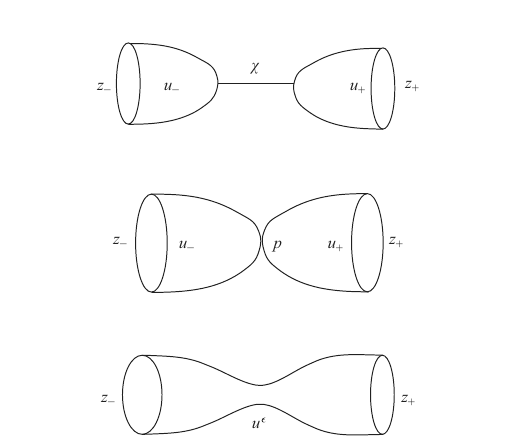
\includegraphics[width=.62\textwidth]{chapters/ch20-pants-product/figures/figure-20-2.png}
 \caption{PSS 方案。}
 \label{fig:20-pss-scheme}
\end{figure}

\subsection{证明的 PSS 方案}

\stfhIndex{I153}{Piwunixin-Salameng-Shiwaci}{皮乌尼欣--萨拉蒙--施瓦茨（Piunikhin--Salamon--Schwarz）}
本小节概述\personPiunikhin{}、\personSalamon{}和\personSchwarz{}对 PSS 映射同构性质的论证；它基于一个
形变，把复合映射
\[
 \Phi\circ\Psi:CF_*(H_+)\longrightarrow CF_*(H_+)
\]
与恒等映射之间建立链同伦。形变过程中涉及三类模空间（见图~\ref{fig:20-pss-scheme}）：
\footnote{译者注：原书此处称形变导向复合映射与恒等映射之间的“chain
isomorphism”，但随后构造的是链同伦并明确写出链同伦公式；译文据此写作“链同伦”。}
\begin{samepage}
\begin{enumerate}[label=(\arabic*)]
\item 圆盘--流--圆盘；
\item 节点\personFloer{}流线；
\item 链映射\personFloer{}流线。
\end{enumerate}
\end{samepage}

以下以 $\lambda\in[-1,1]$ 表示形变参数，使节点位形出现在 $\lambda=0$。只要
$\lambda>0$ 或 $\lambda<0$，形变所涉及的模空间类型相同，故标准论证分别在
$[-1,-\epsilon_0]$ 和 $[\epsilon_0,1]$ 上构造配边。要把配边延拓到整个区间，需要
用 $[-\epsilon_0,\epsilon_0]$ 上的配边连接二者。然而，模空间在 $\lambda=0$ 发生
“相变”，所以先验地只能期望得到\emph{分片光滑}配边；必须证明
$\mathcal M_0\subset\mathcal M^{\mathrm{para}}$ 的\emph{双领口定理}，才能实现 PSS 方案。
从 $-\epsilon_0$ 到 $0$ 的左单侧领口可由有限维构造得到（见 (OhZ11b) 第 9 节）；
$[0,\epsilon_0]$ 上右单侧领口的构造是非平凡的，它基于定理~\ref{thm:20-adiabatic-gluing}，
其证明使用 (OhZ11b) 的绝热退化方法。

应用定理~\ref{thm:20-adiabatic-gluing}，并逐字重复 (OhZ11b) 的论证（该论证又大体
沿用 (PSS96)），可证明下述 (PSS96) 中的同构性质。

\begin{theorem}
\label{thm:20-pss-one-sided-inverse}
令 $(-f;g)$ 为 $M$ 上\personMorse{}函数 $f$ 与度量 $g$ 的通有\personMorse{}--\personSmale{}偶对，
$H^{\mathrm{Morse}}(-f;g)$ 为其\personMorse{}同调。令 $(H,J)$ 为通有的含时周期哈密顿量
$H$ 与 $M$ 上相容殆复结构族 $J=\{J_t\}$。设 $\Psi,\Phi$ 为 (PSS96) 中的 PSS
映射。则存在同态
\[
 \Upsilon_{\mathrm{PSS}}:CF_*(H,J)\longrightarrow CF_{*+1}(H,J)
\]
满足
\begin{equation}
 \Phi\circ\Psi-\operatorname{id}
 =\partial_{(H,J)}\circ\Upsilon_{\mathrm{PSS}}
 -\Upsilon_{\mathrm{PSS}}\circ\partial^{\mathrm{Morse}}_{(-f,g)}.
 \label{eq:20-pss-chain-homotopy}
\end{equation}
\footnote{译者注：原书此式两项之间为减号；本节稍后的链同伦公式却使用加号。
这可能涉及作者的边界算子符号约定，也可能是排印不一致。此外，原书第二项使用
$\partial^{\mathrm{Morse}}_{(-f,g)}$，但 $\Upsilon_{\mathrm{PSS}}$ 的定义域和值域均为
$CF_*(H,J)$，故该复合在类型上也不成立；译文两处均照录。}
特别地，在同调上 $\Phi_*\circ\Psi_*=\operatorname{id}$。
\end{theorem}

这说明 $\Phi_*\circ\Psi_*=\operatorname{id}$。另一个恒等式
$\Psi_*\circ\Phi_*=\operatorname{id}$ 更容易证明；细节见 (OhZ11b) 第 9 节。

\begin{remark}
\label{rem:20-one-jet-datum}
\personFloer{}流线方程解模空间带中部\personMorse{}函数 $\epsilon f$ 的绝热退化，不仅产生 PSS 方案所用
的节点\personFloer{}流线，还产生带一阶喷注数据的节点\personFloer{}流线；该数据反映背景\personMorse{}函数 $f$ 的存在。这在 (OhZ11b) 的尺度依赖粘合中至关重要。
\end{remark}

\subsection{\texorpdfstring{$\Phi_*\circ\Psi_*=\operatorname{id}$}{Phi o Psi = id}：从\personFloer{}经\personMorse{}回到\personFloer{}}

考虑定义在 $\kappa\in[-\infty,1]$ 上的 PSS 形变。固定通有同伦
$(K^\kappa,J^\kappa)$，其中
$K^\kappa=K^\kappa(\tau,t,x)$、$J^\kappa=J^\kappa(\tau,t,x)$，它从
$(K^{\epsilon_0},J^{\epsilon_0})$ 连接到
$(K^1(\tau,t,x),J^1(\tau,t,x))=(H(t,x),J(t,x))$。
固定充分小的 $\epsilon_0>0$ 与充分大的 $\ell_0>0$，把形变分成四段：
\[
 \begin{array}{ll}
 (K^\kappa,J^\kappa),&\epsilon_0\leq\kappa\leq1,\\
 (K_\epsilon,J_\epsilon),&0<\kappa=\epsilon\leq\epsilon_0,\\
 (H^{\rho_-},J^{\rho_-})_{o_-}*(-f,g_{J_0};[-\ell,\ell])_{*_{o_+}}
 (H^{\rho_+},J^{\rho_+}),&-\ell_0\leq\ell<0,\\
 (H^{\rho_-},J^{\rho_-})_{o_-}*(-f,g_{J_0};[-\ell,\ell])_{*_{o_+}}
 (H^{\rho_+},J^{\rho_+}),&-\infty\leq\ell<-\ell_0.
 \end{array}
\]
这里 $(f,J_0;[-\ell,\ell])$ 表示形变
\[
 \ell\in(-\infty,0)\longmapsto(-f,g_{J_0};[-\ell,\ell]),
\]
其中 $f$ 是相对于度量 $g_{J_0}$ 的\personMorse{}函数，我们考虑其在区间
$[-\ell,\ell]$ 上的梯度流线。

以 $\mathcal M_\kappa^{\Psi\Phi}([z_-,w_-],[z_+,w_+])$ 表示对应参数 $\kappa$ 的
位形模空间，以参数化模空间表示整个形变：
\[
 \overline{\mathcal M}_{\Psi\Phi}^{\mathrm{para}}
 ([z_-,w_-],[z_+,w_+];f)
 =\bigcup_{\kappa\in[-1,\infty]}
 \mathcal M_\kappa^{\Psi\Phi}([z_-,w_-],[z_+,w_+]).
\]
\footnote{译者注：本小节开头把参数域写作 $[-\infty,1]$，此处却反向写作
$[-1,\infty]$；随后各段又使用负无穷端与上端 $1$，故两处不能同时成立。译文照录。}
由非退化假设和指标条件，除有限多个点外 $\mathcal M_\kappa^{\Psi\Phi}$ 为空；这些点
位于
\[
 \kappa\in(-\ell_0,-\ell_1)\cup(\epsilon_0,1).
\]
先验地，当 $\kappa\to0$ 时它们可能在 $[-\ell_1,\epsilon_0]$ 内聚集。但对应
$\kappa=0$ 的加强节点\personFloer{}流线模空间的一阶喷注横截性，以及
定理~\ref{thm:20-adiabatic-gluing} \emph{排除}了这种聚集。因此，若取 $\ell_1,\epsilon_0$
充分小，则对所有 $\kappa\in[-\ell_1,\epsilon_0]$ 有
\[
 \mathcal M_\kappa^{\Psi\Phi}([z_-,w_-],[z_+,w_+])=\varnothing.
\]
结合主要粘合紧性结果和定理~\ref{thm:20-adiabatic-gluing}，得到：

\begin{proposition}
\label{prop:20-phi-psi-compactification}
存在常数 $\ell_0,\ell_1,\epsilon_0,\epsilon_1$，使：
\begin{enumerate}[label=(\arabic*)]
\item 若 $\mu_H([z_-,w_-])-\mu_H([z_+,w_+])=-1$，则
$\overline{\mathcal M}_{\Psi\Phi}^{\mathrm{para}}([z_-,w_-],[z_+,w_+])$
是紧零维流形，并且当
$\kappa\in[-\infty,-\ell_0]\cup[-\ell_1,\epsilon_0]\cup[1-\epsilon_1,1]$
时 $\mathcal M_\kappa^{\Psi\Phi}=\varnothing$。
\item 若指标差为 $0$，则
$\overline{\mathcal M}_{\Psi\Phi}^{\mathrm{para}}([z_-,w_-],[z_+,w_+];f)$
是紧一维流形，其边界为
\[
 \begin{aligned}
 \partial\overline{\mathcal M}_{\Psi\Phi}^{\mathrm{para}}
 &=\mathcal M_{\kappa=1}([z_-,w_-],[z_+,w_+])
 \cup\mathcal M_{-\infty}([z_-,w_-],[z_+,w_+])\\
 &\quad\cup\bigcup_{[z,w]}
 \overline{\mathcal M}_{\Psi\Phi}^{\mathrm{para}}([z_-,w_-],[z,w])
 \#\mathcal M_{\kappa=1}([z,w],[z_+,w_+])\\
 &\quad\cup\bigcup_{[z,w]}
 \mathcal M_{\kappa=1}([z_-,w_-],[z,w])
 \#\overline{\mathcal M}_{\Psi\Phi}^{\mathrm{para}}([z,w],[z_+,w_+]),
 \end{aligned}
\]
第一、第二个并分别遍历满足相应指标差为 $-1$ 的 $[z,w]$。
\end{enumerate}
\end{proposition}

命题 (1) 可定义阶数为
$\#\overline{\mathcal M}_{\Psi\Phi}^{\mathrm{para}}([z_-,w_-],[z_+,w_+];f)$
的矩阵系数，从而定义映射
\[
 \Upsilon_{\mathrm{PSS}}^{\Psi\Phi}:CF_*(H)\to CF_{*+1}(H),
\]
其矩阵系数为
\[
 \langle\Upsilon_{\mathrm{PSS}}^{\Psi\Phi}([z_-,w_-]),[z_+,w_+]\rangle
 =\#\overline{\mathcal M}_{\Psi\Phi}^{\mathrm{para}}([z_-,w_-],[z_+,w_+];f).
\]
命题 (2) 对一维模空间边界的描述转化为
\[
 \Phi\circ\Psi-\operatorname{id}
 =\partial\circ\Upsilon_{\mathrm{PSS}}^{\Psi\Phi}
 +\Upsilon_{\mathrm{PSS}}^{\Psi\Phi}\circ\partial.
\]
这完成了同调上 $\Phi_*\circ\Psi_*=\operatorname{id}$ 的证明。

\subsection{\texorpdfstring{$\Psi_*\circ\Phi_*=\operatorname{id}$}{Psi o Phi = id}：从\personMorse{}经\personFloer{}回到\personMorse{}}

对每一对 $p,q\in\operatorname{Crit}f$，考虑参数化模空间
\[
 \overline{\mathcal M}_{\Phi\Psi}^{\mathrm{para}}(p,q)
 =\bigcup_{0\leq R\leq\infty}\mathcal M_R^{\Phi\Psi}(p,q).
\]
定义如下。对每个 $0<R<\infty$，先引入方程
\begin{equation}
 \overline\partial_{(K^R,J^R)}u=0
 \label{eq:20-r-dependent-cr}
\end{equation}
在 $\Sigma$ 上的有限能量解模空间
$\mathcal M_{(2;0,0)}(K^R,J^R)$。这里 $\Sigma$ 是带两个标记点
$\{o_-,o_+\}$ 的\personRiemann{}曲面，满足
$\Sigma\setminus\{o_\pm\}\cong\mathbb R\times S^1$。先以连通和定义\personRiemann{}曲面族 $(\Sigma,j_R)$：
\[
 (D^-,o_-)\cup C_R\cup(D^+,o_+),\qquad
 j_R=j_{D^-}\#j_{C_R}\#j_{D^+},
\]
其中 $C_R=[-R,R]\times S^1$，$j_{C_R}$ 是标准共形结构，$j_R$ 是
$D^-\cup C_R\cup D^+$ 上显然的粘合共形结构。以 $(\tau,t)$ 表示
$D^-\cup C_R\cup D^+\setminus\{o_-,o_+\}$ 上延拓 $C_R$ 标准坐标的共形坐标。

在这些坐标中固定截断函数族
\[
 \chi^R(\tau)=\begin{cases}
 1-\kappa^+(\tau-R),&\tau\geq0,\\
 1-\kappa^-(\tau+R),&\tau\leq0,
 \end{cases}
\]
其中 $1\leq R<\infty$；对 $0\leq R\leq1$ 令 $\chi^R=R\chi^1$。注意
$\chi^0\equiv0$，$\chi^R$ 具有紧支集，并且对任意给定紧子集，当 $R$ 充分大时
$\chi^R\equiv1$。因此，方程~\eqref{eq:20-r-dependent-cr} 在标记点 $o_\pm$ 附近化为
$\overline\partial_{J_0}u=0$。如前定义 $(K^R,J^R)$。

有两个评价映射
\[
 \operatorname{ev}_{o_\pm}:\mathcal M_{(2;0,0)}(K^R,J^R)\to M,
 \qquad\operatorname{ev}_{o_\pm}(u)=u(o_\pm).
\]
记
\[
 \begin{aligned}
 \widetilde{\mathcal M}^-(p;f)
 &=\{\chi:\mathbb R\to M\mid\dot\chi+\nabla(-f)(\chi)=0,
 \ \chi(-\infty)=p\},\\
\widetilde{\mathcal M}^+(q;f)
&=\{\chi:\mathbb R\to M\mid\dot\chi+\nabla(-f)(\chi)=0,
 \ \chi(+\infty)=q\},
\end{aligned}
\]
\footnote{译者注：原书把以上两处映射的类型写成“$\chi:\mathbb R\times M$”，没有
给出值域；由微分方程及端点条件可知应为 $\chi:\mathbb R\to M$，译文据此补正。}
并定义
\[
 \widetilde{\mathcal M}_1^-(p;-f)=\widetilde{\mathcal M}^-(p;-f)\times\mathbb R,
 \qquad
 \widetilde{\mathcal M}_1^+(q;-f)=\widetilde{\mathcal M}^+(q;-f)\times\mathbb R.
\]
$\tau_0\in\mathbb R$ 通过
$(\tau_0,(\chi,\tau))\mapsto(\chi(*-\tau_0),\tau+\tau_0)$ 自由作用，故商
\[
 \mathcal M_1^-(p;-f)=\widetilde{\mathcal M}_1^-(p;-f)/\mathbb R,
 \quad
 \mathcal M_1^+(q;-f)=\widetilde{\mathcal M}_1^+(q;-f)/\mathbb R
\]
\footnote{译者注：原书先以参数“$f$”定义 $\widetilde{\mathcal M}^{\pm}(\cdot;f)$，
但方程已使用 $\nabla(-f)$；紧接着又把同一对象代入参数“$-f$”定义
$\mathcal M_1^{\pm}(\cdot;-f)$。若逐字代入会反转梯度号，故此处存在记号不一致；
译文保留原书记号。}
分别是维数 $\mu_{\mathrm{Morse}}(p;f)$ 与
$2n-\mu_{\mathrm{Morse}}(q;f)$ 的光滑流形。其渐近评价映射
\[
 \operatorname{ev}_+:\mathcal M_1^+(q;-f)\to M,
 \qquad \operatorname{ev}_-:\mathcal M_1^-(p;-f)\to M
\]
的像分别与不稳定流形 $W^u(p;-f)$ 和稳定流形 $W^s(q;-f)$ 一一对应。
\footnote{译者注：原书按 $\operatorname{ev}_+$、$\operatorname{ev}_-$ 的顺序列出
定义域 $\mathcal M_1^+(q;-f)$、$\mathcal M_1^-(p;-f)$，却说其像“分别”为
$W^u(p;-f)$、$W^s(q;-f)$；变量和稳定/不稳定流形均与该顺序不匹配。译文照录。}

定义 $\mathcal M_R^{\Phi\Psi}(p,q;A)$ 为\termFiberProduct{}
\[
 \begin{aligned}
 \mathcal M_R^{\Phi\Psi}(p,q;A)
 &=\mathcal M_1^-(p;-f)_{\operatorname{ev}_-}
 \times_{\operatorname{ev}_{o_-}}\mathcal M_{(2;0,0)}(K^R,J^R;A)\\
 &\qquad{}_{\operatorname{ev}_{o_+}}
 \times_{\operatorname{ev}_+}\mathcal M_1^+(q;-f)\\
 &=\{((\chi_-,\tau_-),u,(\chi_+,\tau_+))\mid
 \chi_-(\tau_-)=u(o_-),\ \chi_+(\tau_+)=u(o_+)\},
 \end{aligned}
\]
并令
\[
 \overline{\mathcal M}^{\Phi\Psi,\mathrm{para}}(p,q;A)
 =\bigcup_{0\leq R\leq\infty}\mathcal M_R^{\Phi\Psi}(p,q;A).
\]
直接计算得到
\[
 \dim^{\mathrm{virt}}\mathcal M_R^{\Phi\Psi}(p,q;A)
 =\mu_{\mathrm{Morse}}(p)-\mu_{\mathrm{Morse}}(q)+2c_1(A).
\]

\begin{proposition}
\label{prop:20-psi-phi-compactification}
取通有偶对 $(f,J_0)$，并令 $0<\epsilon_1<R_1$。
\footnote{译者注：原书在本命题开头先令 $0<\epsilon_1<R_1$，但第 (1) 项又说“存在
某个 $\epsilon_1>0$ 和 $R_1>0$”；证明末还写成相反的 $R_1\leq\epsilon_1$。这些
量词和不等式彼此不容，译文逐处照录。}
\begin{enumerate}[label=(\arabic*)]
\item 若 $\mu_{\mathrm{Morse}}(p)-\mu_{\mathrm{Morse}}(q)+2c_1(A)=-1$，
则存在某个 $\epsilon_1>0$ 与 $R_1>0$，使
$\overline{\mathcal M}^{\Phi\Psi,\mathrm{para}}(p,q;A)$ 是紧零维流形，并且当
$0\leq R\leq\epsilon_1$ 或 $R\geq R_1$ 时
$\mathcal M_R^{\Phi\Psi}(p,q;A)=\varnothing$。
\item 若上述指标为 $0$，则
$\overline{\mathcal M}^{\Phi\Psi,\mathrm{para}}(p,q;A)$ 是紧一维流形，其边界为
\[
 \partial\overline{\mathcal M}^{\Phi\Psi,\mathrm{para}}(p,q;A)
 =\mathcal M_0^{\Phi\Psi}(p,q;A)\cup\mathcal M_\infty^{\Phi\Psi}(p,q;A)
 \cup\bigcup_r\overline{\mathcal M}^{\Phi\Psi}(p,r;A),
\]
\footnote{译者注：原书边界式最后一项只含 $(p,r;A)$，使原先固定的输出 $q$ 消失；
若它描述\personMorse{}破裂，通常还应出现从 $r$ 到 $q$ 的因子。页内资料不足以唯一补全，
译文照录。}
其中最后的并遍历满足
$\mu_{\mathrm{Morse}}(p)-\mu_{\mathrm{Morse}}(r)+2c_1(A)=-1$ 的
$r\in\operatorname{Crit}(-f)$。
\end{enumerate}
\end{proposition}

\begin{proof}
当 $R=0$ 时，方程~\eqref{eq:20-r-dependent-cr} 化为
$\overline\partial_{J_0}u=0$。因为
$\mu_{\mathrm{Morse}}(p)-\mu_{\mathrm{Morse}}(q)+2c_1(A)=-1$ 是
$\mathcal M_0^{\Phi\Psi}(p,q;A)$ 的虚维数，对通有 $(f,J_0)$ 该空间必为空。这里强调，
此模空间只依赖 $(f,J_0)$，故通有性论证可与参数 $R$ 无关地应用。因此当
$R_1\leq\epsilon_1$ 且 $\epsilon_1>0$ 充分小时，同样成立。证明完毕。第 (2) 项留给
读者。
\end{proof}

由 (1) 定义链同伦映射
\[
 \Upsilon_{\mathrm{PSS}}^{\Phi\Psi}:
 CM_*(-f,g_{J_0};\Lambda_\omega)\to CM_{*+1}(-f,g_{J_0};\Lambda_\omega),
\]
其矩阵元为
\[
 \langle\Upsilon_{\mathrm{PSS}}^{\Phi\Psi}(p),q\#(-A)\rangle
 =\sum_{(r,A)}\#\left(\bigcup_r
 \overline{\mathcal M}^{\Phi\Psi,\mathrm{para}}(p,r;A)\right).
\]
\footnote{译者注：原书左端固定 $q$，右端却对 $(r,A)$ 求和又在括号内再对 $r$ 取并，
同时复用 $A$；该矩阵元的下标无法由页内资料唯一重构，译文照录。}

\begin{lemma}
\label{lem:20-zero-end-dimension}
设 $\mu_{\mathrm{Morse}}(p)-\mu_{\mathrm{Morse}}(q)+2c_1(A)=0$。若 $A\neq0$，则除非
$\mathcal M_0^{\Phi\Psi}(p,q;A)=\varnothing$，否则
\[
 \dim\mathcal M_0^{\Phi\Psi}(p,q;A)\geq2.
\]
当 $A=0$ 时，除非 $p=q$，否则
\[
 \dim\mathcal M_0^{\Phi\Psi}(p,q;A)\geq1.
\]
\end{lemma}

\begin{proof}
若 $A\neq0$，则 $(u;o_-,o_+)\in\mathcal M_{(2;0,0)}(K^R,J^R)$ 中的 $u$ 非常值。
定义域 $(\Sigma;o_-,o_+)$ 的共形自同构产生至少实二维族，与指标假设矛盾（半正
情形见 (Fl89b), (FHS95)，一般情形见 (FOn99), (LT98)）。

若 $A=0$，任何 $J_0$-全纯球面都为常值，相应位形
$(\chi_-,\text{常值},\chi_+)$ 因而成为完整梯度流线
$\chi=\chi_-\#\chi_+$。除非 $\chi$ 为常值（即 $p=q$），否则 $\mathbb R$-平移产生
至少一维族，再次与指标假设矛盾。
\end{proof}

现在可完成恒等式
\begin{equation}
 \Psi\circ\Phi-\operatorname{id}
 =\Upsilon_{\mathrm{PSS}}^{\Phi\Psi}\partial^{\mathrm{Morse}}_{(-f,g_{J_0})}
 +\partial^{\mathrm{Morse}}_{(-f,g_{J_0})}\Upsilon_{\mathrm{PSS}}^{\Phi\Psi}
 \label{eq:20-psi-phi-chain-homotopy}
\end{equation}
的证明。先验地，命题~\ref{prop:20-psi-phi-compactification} 只给出
\[
 \sum_{q,A}\langle(\Psi\circ\Phi-\operatorname{id})(p),q\#(-A)\rangle
 =\sum_{q,A}\left\langle
 \Upsilon_{\mathrm{PSS}}^{\Phi\Psi}\partial^{\mathrm{Morse}}_{(-f,g_{J_0})}(p)
 +\partial^{\mathrm{Morse}}_{(-f,g_{J_0})}\Upsilon_{\mathrm{PSS}}^{\Phi\Psi}(p),
 q\#(-A)\right\rangle.
\]
但上述引理蕴含
\[
 \langle(p),q\#(-A)\rangle=0,
\]
除非 $A=0$ 且 $p=q$。这便证明了~\eqref{eq:20-psi-phi-chain-homotopy}。
